%\title{SWEETcam submission for IEEE Computer}

%%
%% Draft version 2.0
%%
%% Authors:
%% Kevin Abas
%% Caio Porto
%% Katia Obraczka 
%%


%%*************************************************************************
%% Legal Notice:
%% This code is offered as-is without any warranty either expressed or
%% implied; without even the implied warranty of MERCHANTABILITY or
%% FITNESS FOR A PARTICULAR PURPOSE! 
%% User assumes all risk.
%% In no event shall IEEE or any contributor to this code be liable for
%% any damages or losses, including, but not limited to, incidental,
%% consequential, or any other damages, resulting from the use or misuse
%% of any information contained here.

%%*************************************************************************

\documentclass[journal,transmag]{IEEEtran}

% *** GRAPHICS RELATED PACKAGES ***
%
\usepackage{graphicx}
\ifCLASSINFOpdf

\else

\fi

% *** ALIGNMENT PACKAGES ***
%
\usepackage{array}

% *** PDF, URL AND HYPERLINK PACKAGES ***
%
\usepackage{url}
% url.sty was written by Donald Arseneau. It provides better support for
% handling and breaking URLs. url.sty is already installed on most LaTeX
% systems. The latest version and documentation can be obtained at:
% http://www.ctan.org/tex-archive/macros/latex/contrib/url/
% Basically, \url{my_url_here}.

% correct bad hyphenation here
\hyphenation{op-tical net-works semi-conduc-tor}

% ** BIBTEXT PACKAGE **
\usepackage{cite}

% ** CAPTION PACKAGE **
\usepackage{caption}
%%----------------------------------------------------------------------

\begin{document}


%% ***********************  THE TITLE **********************************

\title{Efficient Smart Camera Networks For Public Safety}


%% ***********************  AUTHORS ************************************

\author{\IEEEauthorblockN{Kevin Abas\IEEEauthorrefmark{1},
Caio Porto\IEEEauthorrefmark{2},
Katia Obraczka\IEEEauthorrefmark{1}}
\IEEEauthorblockA{\IEEEauthorrefmark{1}School of Engineering,
University of California Santa Cruz, CA 95064 USA}
\IEEEauthorblockA{\IEEEauthorrefmark{2}Escola Politecnica ´
Avenida Athos da Silveira Ramos ´
Rio de Janeiro, 21941-909, Brazil}
}


%% ***********************  AUTHORS ************************************

\IEEEtitleabstractindextext{%
\begin{abstract}
\textit{Abstract} \-- With the advancement of wireless smart camera platforms many systems have emerged offering more 
efficient surveillance solutions for public spaces. After surveying more recent surveillance systems from the research community
a classification is created to better help us understand what the future holds in this field.
\end{abstract}


%% ********************** IEEE KEYWORDS ********************************

\begin{IEEEkeywords}
Wireless sensor networks, Smart camera networks, Computer vision, Sensor networks, Human safety
\end{IEEEkeywords}}



%% Title Configurations (From Template)
\maketitle
\IEEEdisplaynontitleabstractindextext
\IEEEpeerreviewmaketitle


%% *********************  BEGIN PAPER **********************************

\section{Introduction}

\IEEEPARstart{T}{his} paper discusses an overview of how Smart Camera Networks are changing surveillance systems of today.\\
\-- Goals of the paper, What problems this papers solves, background, motivation \\
\-- discuss Wireless sensor networks in general and how data rich video sensor are\\
\-- Some things current Smart Camera networks assist with when it comes to 
surveillance and crime detection nodes. \\

%%Requirements for today's wireless Smart Camera Networks

\section{Wireless Smart Camera Surveillance}
Researchers and Commercial companies are designing wireless smart camera networks in surveillance applications to prevent crimes, detect environmental emergencies,
monitor behavior of the elderly, and track vehicular traffic in public spaces. Many camera platforms have been designed to meet strict hardware requirements
~\cite{Flexi-WVSNP} for wireless deployment in surveillance systems. However, different requirements must be stated when looking at the application specific 
scenario of surveillance in public spaces. To understand how these state of the art systems are improving on designs of the past, one must define what makes these
surveillance systems "smart". These smart camera network systems have common goals when it comes creating more efficient surveillance applications. First, the issue 
of network resource utilization is an issue all systems need to consider if those surveillance systems are to be scalable in crowded wireless deployment 
scenarios. Then in almost every application considering power consumption of each node is very important if one is give an analysis of the systems 
efficiency. If these systems are to be monitoring public spaces the smart camera networks need to be keeping the data recorded secure and also
ensuring that the data recorded is actually quality information that could be used by officials. 

\subsection{Bandwidth Efficiency}
Video data is rich with useful information that other sensor sources can’t provide, however video data quickly becomes very large in size as time goes 
on.Nodes competing for network connectivity while maintaining quality on live video feed can soon become a problem as the network grows or if other 
nodes not in the system share the connection. One way to combat this is by assuring the data recorded is useful and actually recording video data that 
can be used to do detection of events by doing in network processing ~\cite{Citric}.\\
Taking advantage of multiple cameras is a very useful method to determine not only which node has the best view of the object, but also if the overlapping
video footage can be combined to provide more useful data. Extensive research has been done on both bandwidth and energy efficiencies of wireless
smart camera networks that make use of overlapping footage ~\cite{AccLatEnergy}.


\subsection{Lowering Power Consumption}
When discussing wireless sensor networks , power consumption is always brought up as a concern in deployment and scalability. Smart camera networks are 
no different, and many researchers have discussed methods to design nodes that consume less power. One such method would be to limit the amount of time 
a camera needs to actually be powered on, and rely on more low power sensors to trigger a wake up. Using this sensor fusing technique allows the system
to operate a different power consumption states . Such states must be carefully looked at and many researchers 
consider every level of operation of each camera node ~\cite{AccLatEnergy}~\cite{EnergyCons}. Making Smart hardware choices, such at choosing low power communication
options such as 802.15.4, can also have a large effect on how much power the system uses.

\subsection{Quality of data recorded}
Recording live high-resolution data all the time with no inference will soon become a thing of the past. Every second of video recorded counts when the 
surveillance system scales to much larger deployments such as in smart cities~\cite{HuSIMS}. Doing local proccessing and decision making first can have 
a huge change on the amount of data that actually needs to be transmitted and archived. Whether it is event detection or object identification, preventing 
false alarms by checking the data locally can be very helpful. The research area of computer vision has grown at a very fast rate and only in the past few years
are we seeing wireless surveillance systems adopt these sophisticated algorithms.


\twocolumn[
\section{Classifying Smart Wireless Surveillance Systems}
\begin{center}
\captionof{table}{A taxonomy of current research surveillance systems that use wireless smart cameras.}
\resizebox{\textwidth}{!}{%
\begin{tabular}{| l | p{3cm} | l | p{3cm} | p{2cm} | p{3cm} | p{3cm} | l| p{3cm} |}
    \hline
    System & Energy Efficiency & Multimodal & Bandwidth Efficiency & Wireless & Video Analysis & System Software & Multicamera & Security \\ \hline
    
    Citric & sleeping nodes, only wake on presence of objects & Audio & In-network image processing, small image size & 802.15.4 and Bluetooth
     & . & Embedded Linux & Yes & Pre-processing of data at node \\ \hline
    
    HuSIMS & . & . & .  & . & . & . & . & .  \\ \hline
    
    OmniEye & . & . & .  & WiPort 802.11b/g & . & . & . & .  \\ \hline
    
    Wi-FLIP & . & . & .  & . & . & . & . & .  \\ \hline
    
    SensEye & . & . & .  & . & . & . & . & .  \\ \hline
    
    DTN-Citric & . & . & .  & . & . & . & . & .  \\ \hline
    
    Flexi-WVSNP & . & . & .  & . & . & . & . & .  \\ \hline
    
    MeshEye & . & . & .  & . & . & . & . & .  \\ \hline
	
\end{tabular}}
\end{center}
]

\subsection{Energy Efficiency}
\subsection{Sensor Fusion}
\subsection{Network Load and Scalability}
\subsection{Wireless Communication}
\subsection{Computer Vision in Surveillance}
By the computer vision side, we can see that the background subtraction is the most used method to detect moving objects with single cameras in a 
real-time world. There are different algorithms to implement it, with different computer efficiencies and accuracies, what can make each one more
suitable for each system. Methods like Mixture of Gaussians (MoG) or simple frame differencing are largely used, but the problem with these methods is
their computational efficiency. In ~\cite{CS-MoG} it is shown the possibility of having a low power and computationally efficient (up to 5 times
faster) system based on background subtraction using a known method: Compressed Sensing. Using CS is possible to compress the image, in other words,
reduce the amount of data to be processed, while retaining much of the original image. The compressed image can be submitted to a MoG algorithm to
detect the objects on the scene with a lower solution complexity. The results shown a very efficient system, that they called CS-MoG, with an accuracy
very close to a system that uses MoG only.

The Citric system one that resembles ~\cite{CS-MoG} by the steps that are used in the object detection. At first they make a comparison of
computational efficiency relative to the complexity of compressing and uncompressing using JPEG and Compressed Sensing, resulting in a better
performance of the CS  for uncompressing. After that they use frame differencing to do background subtraction and then track the objects and store
their tracks. On the HuSIMS system they take one step further after tracking the objects, it is implemented an algorithm that is able to trigger alarms
if something looks irregular. After doing the object tracking they are able to define regions, representing where the most common tracks pass by, and
sinks, representing places where the objects usually appear or disappear from the scene. Having these two defined sections there is an algorithm
capable of analyzing the image and verify, for example, if the objects of a certain type is following the expected region for its type, or if the
object went from one sink to another. In a case where one of these predicted behaviors looks different, an alarm is triggered notifying that a problem
could happened. \\ \\
A problem very common with single camera systems is the object occlusions that can occurs when an object cross by other moving or static objects. A
good method for this case is shown in ~\cite{Occlusion}. After a background subtraction using the Approximate Median Filter to detect the objects, they
are classified accordingly to the change of their shape through the time. It is used a Kalman filter to predict the position of the objects and then 
compare the current positions with the predicted ones through an algorithm that allows the system to classify the object as a single person or a group 
of people. The particular characteristic of this algorithm is the ability to track objects with complete occlusion for a long duration.
Different implementations for security camera networks are emerging, each one with its characteristics, performance and advantages. By looking at all 
the implementations already said, we can say that a good system could be made by the union of all these methods, if performances wasn’t a constraint, 
because in most of them it is used the same base algorithm but with different securities and tracking objectives. Create an efficient system could mean 
a hybrid one.
\subsection{Management Software}
\subsection{Multi-camera Advantages}
\subsection{Securing The Data}


\section{The SWEETcam Project}
As a proof of concept we've designed our own wireless smart camera node to help improve safety on campus. we've made use of the very popular RaspberryPi for
its powerful processing capabilities, low cost, and its capability to run Linux. Some components we found very useful to achieve our goals including the 
Broadcom SOC(System On a Chip), 700 MHz ARM processor, and its very own GPU for video processing. With the system running Linux, it was very easy for us to
make use of many computer vision libraries already developed for Linux systems.\\
We developed using the newly released Raspberry Pi camera module, which has an available API in C language and is capable of capturing 1920x1080 resolution
color images with 30 fps rate. For the image processing, we chose the Open Source Computer Vision Library (OpenCv). Our computer vision system is developed in 
C++ for better integration between the OpenCV and the API.
\subsection{Energy Harvesting}
Researchers agree that one way to combat the problems of lifetime performance with battery powered wireless sensor nodes is by making use of energy-harvesting
capabilities~\cite{EnergyHarvesting}. We plan on achieving this with our system by using current solar technologies to recharge the camera's local battery. 
Doing this we hope our system will require much less maintanence and remove any requirements for node placement near power grids.

\subsection{Image Processing}
\- Considering the constraints of the system in terms of price and hardware, it is used techniques of background subtraction to do the object detection.
When started, the program keep taking pictures and process them using Mixture of Gaussian (MoG) method by Stauffer and Grimson. With the foreground in
hands we find the contours and then a bounded box is applied following the contours' limit. To remove some noise and false detection a step is added to 
ignore objects of small size. The object classification is the most processor consumption  processes for most of the pedestrian detection systems, 
because it is used training techniques to classify the objects based on a previous stored database. In our case, to reduce the process we classify the 
objects by looking at their dimensions, they are classified as human if the height is two times bigger than the width we classify as a person. \\
\begin{figure}[h!]
\centering
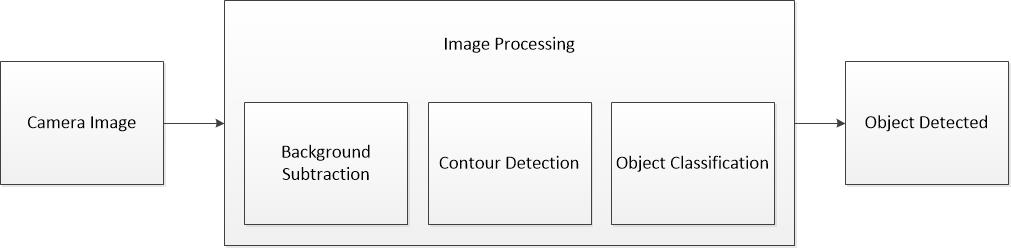
\includegraphics[scale=0.3]{imageprocessing.jpg}
\end{figure}	
\- This light system can generate some false alarms, but in association with the whole system, and its sensors, it can be improved for a better
performance. There are other more robust object detection methods that could be used, but we would have a very low fps rate. 

\subsection{Tracking Object Behavior}
Researchers in the computer vision  field are now moving to not only detect objects and their movements, but to then infer a given behavior is being displayed.
Looking for patterns in the way objects move will help us make better assumptions about what those objects are doing at a more generic level. Using this
information we can do better event detection for specific occurrences and tag the video recorded accordingly. For example, video data that specifically states
it is a recording of a person by a bike rack late in the evening is much more useful that video recorded of just a person.


\section{Future Directions and Lessons to take away}
\-- Discuss research that has been proposed in the area and that is just beginning to be implemented or hasn't yet at all.\\

\-- just so it compiles here are the references to be used:
~\cite{HuSIMS}
~\cite{Citric}
~\cite{OmniEye}
~\cite{DTNSmartCamera}
~\cite{SensEye}
~\cite{WiFLIP}
~\cite{AccLatEnergy}
~\cite{MeshEye}
~\cite{EnergyCons}
~\cite{Flexi-WVSNP}

%% *************************  END PAPER **********************************


% Can use something like this to put references on a page
% by themselves when using endfloat and the captionsoff option.
%\ifCLASSOPTIONcaptionsoff
%  \newpage
%\fi


%% ******************  REFERENCE SECTION **********************************

\bibliography{Bib.bib}{}
\bibliographystyle{plain}


%% ******************  AUTHOR BIOGRAPHIES *********************************

\begin{IEEEbiographynophoto}{Kevin Abas}
is a graduate student at Univeristy of California Santa Cruz. His research
interests include wireless sensor networks, computer networking, and embedded
systems. He recieved his BSc in computer engineering from University of
California Santa Cruz. Contact him at kabas@soe.ucsc.edu.
\end{IEEEbiographynophoto}

\begin{IEEEbiographynophoto}{Caio Porto}
Biography text here.
\end{IEEEbiographynophoto}

\begin{IEEEbiographynophoto}{Katia Obraczka}
Biography text here.
\end{IEEEbiographynophoto}

\end{document}

%%------------------------------------------------------------------------

